\section{Methodology}

This section will describe the methods used to improve the data quality of the Anatomy Registers dataset. All analysis work done was conducted using the Python programming language, specifically, the data processing library \texttt{pandas}. The appendices contain the complete analysis files.

\subsection{Introduction to the dataset}

The Anatomy Registers of The University of Sydney Medical School are a significant data repository that record the sourcing of human bodies for anatomical study from 1883 to present. Detailed records pertaining to the 7609 bodies received between 1883 to 1983 were transcribed into a digital dataset \parencite{rebekah_jenkin} and were deidentified for use in this project in accordance with ethics (approval number 2017/898).

The data, when contextualised with historical events, legal changes, and shifts in medical practices, allows for a comprehensive understanding of how societal values and norms influenced medical science. For example, in part due to a ``lack of public awareness of the value and importance of donating bodies for dissection'' \parencite{rebekah_jenkin}, there was an extreme shortage of bodies for anatomical dissection during the 1940s and 1950s (Figure \ref{fig:ida-by-year}). Additionally, the dataset reveals a predominant male to female ratio, reflecting the gender disparities in residents of the asylums of the time (Figure \ref{fig:ida-by-sex}). 

\begin{figure}[p]
    \centering
    \caption{Number of entries in USYD Anatomy Registers by year}
    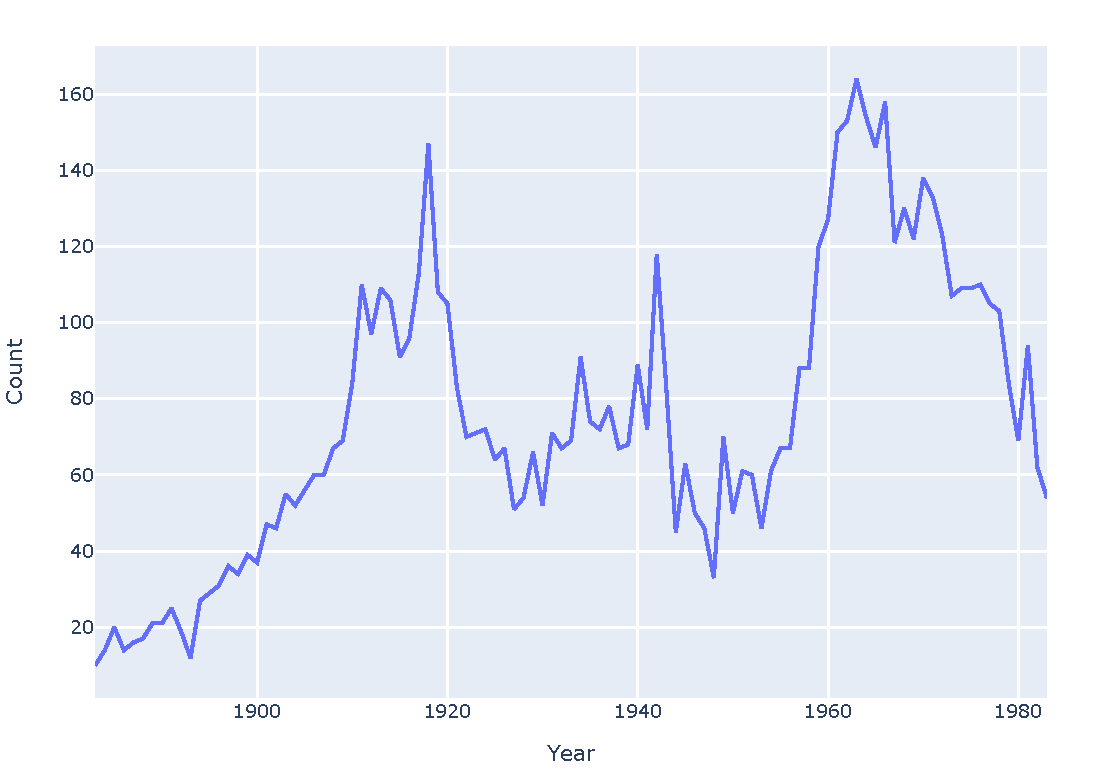
\includegraphics[width=0.9\textwidth]{REPORT/img/data_by_year.pdf}
    \label{fig:ida-by-year}
\end{figure}

\begin{figure}[p]
    \centering
    \caption{Sex of bodies received over time}
    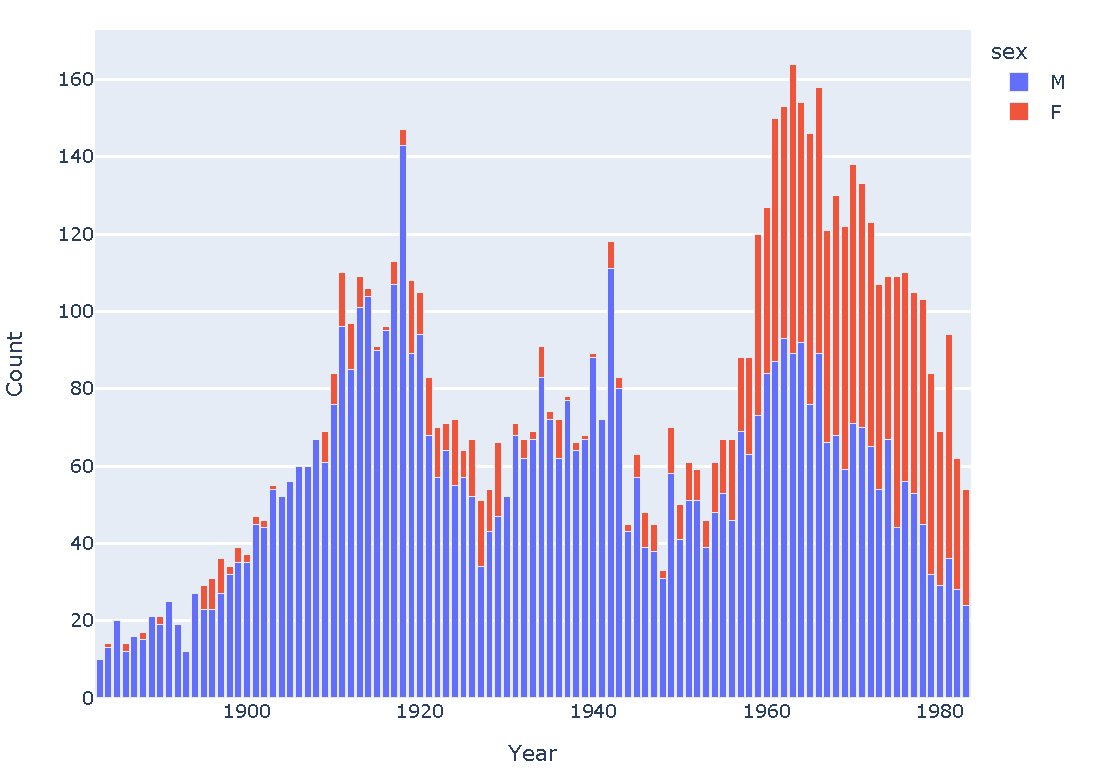
\includegraphics[width=0.9\textwidth]{REPORT/img/data_by_sex.pdf}
    \label{fig:ida-by-sex}
\end{figure}

\subsection{Data verification and validation}\label{subsec:data-v-v}

Data quality can broadly be determined through three factors: (a) data completeness; (b) data consistency; and (c) data validity. 

%%%%%%%%%%%%%%%%%%%%%%%%%%%%%%%
\subsubsection{Data completeness}
%%%%%%%%%%%%%%%%%%%%%%%%%%%%%%%

Data completeness refers to the extent that all expected records and attributes are present in a dataset. Initially, several of our attributes contained missing values (see Table \ref{tab:missing-values}). 


\paragraph{Imputing missing values} Over 2403 entries in the dataset were missing a date of death. However, there were zero missing entries for the date of reception. The date of reception was usually on, or close to (two to three days after) the patient's death. Therefore, the date of reception values were used to impute the missing values of the date of death attribute.

\begin{table}[p]
\centering
\caption{Missing values for attributes in the Anatomy Registers dataset before and after data cleaning}
\label{tab:missing-values}
\singlespacing
\begin{tabular}{@{}lrr@{}}
\toprule
\textbf{Attribute}                        & \textbf{NULL entries before cleaning} & \textbf{NULL entries after cleaning} \\ \midrule
year                    & 0                               &  0                             \\
id                      & 0                               &  0                             \\
sex                     & 5                               &  0                             \\
age                     & 10                              &  0                             \\
death\_date             & 2436                            &  0                             \\
reception\_date         & 0                               &  0                             \\
return\_date\_sepulture & 1680                            &  1673                          \\
burial\_date            & 4408                            &  4394                          \\
death\_place            & 6                               &  0                             \\
place\_code             & 0                               &  0                             \\ \bottomrule
\end{tabular}
\end{table}

\paragraph{Removing entries with missing values} 15 cases had missing values for age, sex or place of death.  As these characteristics could not be imputed from other information, these entries were removed from the dataset. 

%%%%%%%%%%%%%%%%%%%%%%%%%%%%%%%
\subsubsection{Data consistency}
%%%%%%%%%%%%%%%%%%%%%%%%%%%%%%%

Data consistency refers to the dataset adhering to a set of rules and formats. More practically, it involves ensuring each attribute in a dataset fits the most precise datatype it can.

\paragraph{Checking dates}{A regular expression (regex) was utilised to check if dates were in the standard DD/MM/YYYY format.
\begin{equation}
    \texttt{\textasciicircum(0?[0-9]|[12]\textbackslash d|3[01])\/(0?[0-9]|1[0-2])\/(000\textbackslash d|00\textbackslash d\{2\}|0\textbackslash d\{3\}|1\textbackslash d\{3\}|2000)\$}
\end{equation}

Some of the erroneous entries discovered through this method can be seen in Table \ref{tab:error-dates}. In total there were 21 such entries, ranging from a missing forward slash (``/'') in the date to the word ``missing'' or ``[blank]'' being used to indicate a missing value. These entries were then individually corrected by hand.}

\begin{table}[htbp]
\centering
\caption{A few erroneous date entries from each date column}
\label{tab:error-dates}
\begin{tabular}{@{}cllll@{}}
\toprule
\textbf{id} & \textbf{death\_date} & \textbf{reception\_date} & \textbf{return\_date\_sepulture} & \textbf{burial\_date} \\
\midrule
1898 & 25/1/2020 & \ldots & \ldots & \ldots \\
5014 & 26/87/1961 & \ldots & \ldots & \ldots \\
5044 & 20/11/9161 & \ldots & \ldots & \ldots \\
7116 & 5/101977 & \ldots & \ldots & \ldots \\
1727 & \ldots & missing & \ldots & \ldots \\
2408 & \ldots & 23 /4/1925 & \ldots & \ldots \\
2644 & \ldots & \ldots & crossed out 27/9/1929 & \ldots \\
3184 & \ldots & \ldots & [blank] & \ldots \\
3185 & \ldots & \ldots & [blank] & \ldots \\
3203 & \ldots & \ldots & [blank] & \ldots \\
6726 & \ldots & \ldots & \ldots & 04/04//1975 \\
\bottomrule
\end{tabular}
\end{table}


%%%%%%%%%%%%%%%%%%%%%%%%%%%%%%%
\subsubsection{Data validity}
%%%%%%%%%%%%%%%%%%%%%%%%%%%%%%%

Data validity refers to the data accurately representing the real-world values it is supposed to depict -- i.e. the values in the dataset should make sense. Some of the checks conducted are listed below:
\begin{itemize}
    \item Checking the range of \texttt{death\_date} and \texttt{reception\_date} (should be between 1883 and 1983)
    \item Checking that \texttt{death\_date} and \texttt{reception\_date} were no longer than 10 days apart
    \item Checking that \texttt{death\_date} is always less than or equal to \texttt{reception\_date}
\end{itemize}

56 invalid entries were found due to the above checks, mostly due to typos when entering dates. Most of these were corrected by double-checking with the original sources; a few were inferred through looking at surrounding entries for the correct values for day, month, or year.

\subsection{Data transformation}

It is difficult to apply traditional verification techniques such as those discussed in the previous section to the cause of death and place of death columns:

\begin{enumerate}
\item Cause of death and place of death are unstructured text attributes (unlike year, age, and dates).
\item Legislation mandated the maintenance of cause of death and place of death records but did not specify the level of detail required (see the Anatomy Acts of 1881, 1901, and 1977).
\item Medical advancements over the 20th century led to increasingly precise causes of death, with later entries often including detailed tertiary diagnoses.
\end{enumerate}

These attributes are therefore difficult to validate or analyse in their raw form. Hence, \textit{data transformation} was used in order to make programmatic analysis more feasible. Transforming the place of death attribute was our focus for this semester-long project.

%%%%%%%%%%%%%%%%%%%%%%%%%%%%%%%
\subsubsection{Categorising place of death}
%%%%%%%%%%%%%%%%%%%%%%%%%%%%%%%

Regular expressions and keyword analysis techniques were used to extract $\sim$7000 entries into 9 categories based on their place of death (see Table \ref{tab:categories}). For example, the following set of rules were developed to extract private residences:

\begin{table}
    \centering
    \caption{Categories extracted from the place of death attribute in the Anatomy Registers}
    \label{tab:categories}
    \begin{tabular}{ll}
        \toprule
        \textbf{Category} & \textbf{Classification criteria} \\
        \midrule
        Private residence & A private address (commencing with a street, flat, or unit number) \\
        Aged care & Locations containing ``Nursing'', ``Convalescent'', ``Aged Care'', \ldots \\
        Hospice & Locations containing ``Hospice'' + some known hospices \\
        Private hospital & Locations containing ``Private Hospital'' or ``surgery'' \\
        Public hospital & All hospitals without ``private'' in their name\\
        Public asylum & Macquarie St, Liverpool, George St, Rockwood \\
        Public mental asylum & Newingtown + locations containing ``mental asylum'' or ``psychiatric'' \\
        Aged 2 and under & Currently coded 70 \\
        Morgues & Locations containing ``morgue'' \\
        Other & Other \\
        \bottomrule
    \end{tabular}
\end{table}

\begin{enumerate}
    \item The location starts with ``flat'', ``unit'', ``lot'', or contains ``at home'' e.g. ``Flat 73, Darley St, Darlinghurst''
    \item The location starts with a digit, and also contains an address suffix e.g. ``5 York Rd, Bondi Junction''
\end{enumerate}

These rules were converted into regular expressions, and any entries which matched the expressions were categorised as ``private residence.'' A similar procedure was then repeated for each other category, such as ``private hospital'' or ``aged care''.

%%%%%%%%%%%%%%%%%%%%%%%%%%%%%%%
\subsubsection{Extracting suburbs from place of death}
%%%%%%%%%%%%%%%%%%%%%%%%%%%%%%%

In order to pursue a geographical analysis of the Anatomy Registers dataset, it was important to extract some form of location data from the place of death attribute. The most straightforward approach was to extract the suburb name, as it commonly appeared in the unstructured entries of both private residences and other categories of institutions.

A secondary dataset was first sourced which contained the names and geographical boundaries of all 4615 localities in NSW (see Tables \ref{tab:suburb-dataset-details} and \ref{tab:suburb-dataset-head}). Any suburb name present in each place of death entry was then extracted from the records using regular expressions.

\begin{table}[htbp]
\centering
\caption{Attribution details of the NSW Localities dataset}
\label{tab:suburb-dataset-details}
\begin{tabular}{@{}ll@{}}
\toprule
\textbf{Attribute}         & \textbf{Details} \\
\midrule
Dataset name               & NSW Local Government Areas - Geoscape Administrative Boundaries \\
Source                     & Data originally found on data.gov.au. Link here: \url{https://shorturl.at/DMbhb}\\
Attribution                & Licensed by the Commonwealth of Australia under Creative Commons \\
                           & Attribution 4.0 International licence (CC BY 4.0). \\
Last updated               & 27/02/2024 \\
\bottomrule
\end{tabular}
\end{table}

\begin{table}[htbp]
\centering
\caption{First few rows of the NSW Localities dataset}
\label{tab:suburb-dataset-head}
\begin{tabular}{@{}ll@{}}
\toprule
\textbf{suburb}      & \textbf{geometry}      \\ \midrule
Aarons Pass & \texttt{POLYGON (...)} \\
Abbotsbury  & \texttt{POLYGON (...)} \\
Abbotsford  & \texttt{POLYGON (...)} \\
Abercrombie & \texttt{POLYGON (...)} \\ 
Abercrombie River & \texttt{POLYGON (...)} \\
\ldots & \ldots \\ \bottomrule
\end{tabular}
\end{table}

Interestingly, 950 entries from the dataset contained more than one suburb; examples of these can be seen in Table \ref{tab:extract-all-suburbs}. This was mostly for the following reasons:
\begin{enumerate}
    \item An institution contains a suburb in its name but is physically addressed in a different suburb e.g. ``Berrima District Hopsital, Bowral'';
    \item A street shares its name with a suburb e.g. ``Clovelly Rd'';
    \item A combination of the above, often leading to three extracted suburbs e.g. ``Ryde Hospital, Denistone Rd, Eastwood''.
\end{enumerate}

\begin{table}[htbp]
\centering
\caption{A select few examples of place of death entries containing multiple suburbs}
\label{tab:extract-all-suburbs}
\resizebox{\textwidth}{!}{%
    \begin{tabular}{@{}lllll@{}}
    \toprule
    \textbf{id} & \textbf{death\_place} & \textbf{suburb\_1} & \textbf{suburb\_2} & \textbf{suburb\_3} \\ \midrule
    5122 & Corner Clovelly Rd \& Glebe Rd Randwick & Clovelly & Glebe & Randwick \\
    5533 & Berrima District Hospital, Bowral & Berrima & Bowral & - \\
    7567 & Ryde Hospital, Denistone Rd, Eastwood & Ryde & Denistone & Eastwood \\
    7596 & St George Nursing Home, 3 Verdun St, Bexley & St George & Bexley & - \\
    7598 & Kilbride Nursing Home, Appin Rd, Campbelltown & Appin & Campbelltown & - \\ \bottomrule
    \end{tabular}
}
\end{table}

These entries were cleaned programmatically by (a) checking if all classifications of an entry were identical and selecting any one of these classifications, and (b) if the place of death was an address, selecting the suburb which was extracted from the record \textit{last}, as the suburb always comes after the street name and institution name in an address. These steps correctly assigned over 800 of the 950 multiply assigned entries in the dataset.

The remaining entries which could not be condensed through the above procedure were entries with typos, such as ``2 balmoral \textit{avemue} croydon park''; conjunct entries, such as ``hornsby hospital \textit{from} oatlands nursing home dundas''; or institutions which had multiple suburbs in their names, such as ``\textit{ryde} district soldiers memorial hospital \textit{eastwood}''. These last entries were classified manually using a data entry UI created using Jupyter Notebook widgets (see Figure \ref{fig:data-entry-ui}).

\begin{figure}
    \centering
    \caption{Data entry UI made to classify entries manually}
    \label{fig:data-entry-ui}
    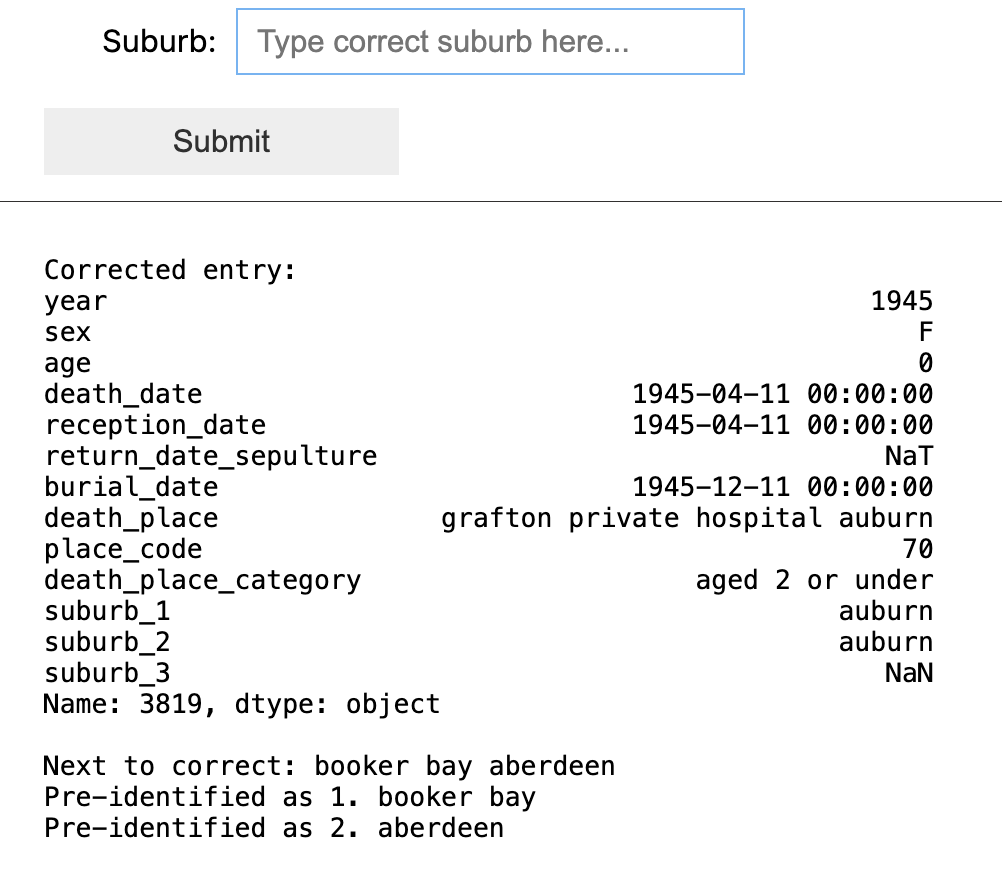
\includegraphics[width=0.6\textwidth]{REPORT/img/data_entry_ui.png}
\end{figure}

Finally, there were 478 entries in the dataset that did not contain any suburbs at all. A majority of these were hospital names, such as ``callan park mental hospital'' or ``dalcross private hospital'', and many contained misspelled suburbs which were unable to be picked up through the regex checker, such as ``wallandra private hospital \textit{marrickvillle}'' or ``outside 1018 francis avenue \textit{brightonlesands}''. These were also manually classified using a modified version of the data entry UI from Figure \ref{fig:data-entry-ui}.

After this process, there were only 86 entries in the dataset (1.33\%) which did not receive a suburb classification. As seen in Figure \ref{fig:missing-suburbs}, about two-thirds of the remaining entries can be attributed to deaths at unspecified morgues, and a large majority of the remaining one-third entries were neonatal deaths which did not routinely include a place of death in the record associated with their receipt by the Medical School. These 86 entries were subsequently dropped from the dataset in order to facilitate an accurate merge with the geographical dataset.

\begin{figure}
    \centering
    \caption{Categories of entries with missing suburb classifications}
    \label{fig:missing-suburbs}
    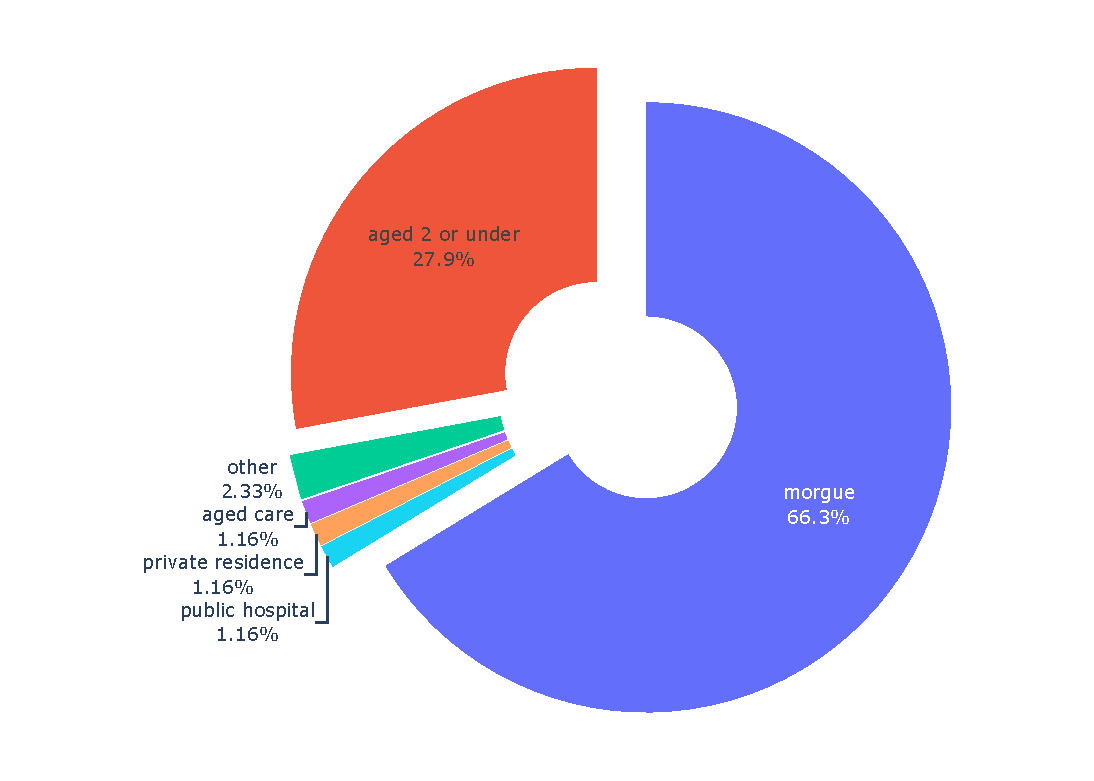
\includegraphics[width=0.9\textwidth]{REPORT/img/missing_suburbs.pdf}
\end{figure}

\paragraph{Merging with NSW geographical dataset}{When first exploring the geographical dataset, it was noted that there were 202 localities across New South Wales with the same name. This would present a significant issue when matching a suburb from the anatomy records to a suburb in the table. In order to deal with this, the Anatomy Registers dataset was first merged with the NSW Localities dataset using a \texttt{LEFT JOIN} in order to retain any duplicates. The dataset was then queried to extract any duplicated suburbs, outputting:
\begin{APAenumerate}
    \item Summer Hill (Inner West $\cdot$ Hunter Region)
    \item Punchbowl (Canterbury-Bankstown $\cdot$ Northern Rivers Region)
    \item Enmore (Inner West $\cdot$ New England Region)
    \item Darlington (Inner West $\cdot$ Hunter Region)
    \item Budgewoi
\end{APAenumerate}

After plotting the duplicates on a map, it was found that Summer Hill, Punchbowl, Enmore, and Darlington were all inner city suburbs having rural villages sharing their name. It was confirmed through corroborating their place of death entries that these patients were not sourced from their rural counterparts. Therefore, the duplicate entries closest to Sydney city were chosen to remain in the dataset.

Lastly, Budgewoi is a coastal town which is naturally divided into two by the Budgewoi Lake causing the duplicate suburb name. One Budgewoi geometry was chosen at random to remain in the dataset.
}

\subsection{Final dataset}

Ultimately, the work conducted in this section led to a cleaned, verified, and useable dataset containing 7510 entries (98.7\% of the original dataset) with nine original and three new attributes (see Table \ref{tab:full-schema}). The quality and utility of the Anatomy Registers dataset was significantly enhanced through employing data verification, validation, and transformation techniques. Furthermore, each step -- from ensuring data completeness to extracting geographical information -- was not only important in preparing the dataset for detailed analysis, but also served as a valuable case study in techniques that can be employed when handling archival data from other sources. 

\begin{table}[ht]
\centering
\caption{Schema of the Anatomy Registers dataset (* indicates a column not present in the original dataset)}
\label{tab:full-schema}
\begin{tabular}{llrl}
\toprule
\textbf{Attribute Name} & \textbf{Data Type} & \textbf{Missing} & \textbf{Description} \\
\midrule
id                      & Integer            & 0                      & Unique identifier for each entry \\
year                    & Integer            & 0                      & Year the body was received \\
age                     & Integer            & 0                      & Age at the time of death \\
death\_date             & Date               & 0                      & Date of the donor's death \\
reception\_date         & Date               & 1                      & Date body was received at the school \\
return\_date\_sepulture & Date               & 1645                   & Date body was returned for burial \\
burial\_date            & Date               & 4353                   & Date of the body's burial \\
death\_place            & String             & 0                      & Location of death \\
place\_code             & String             & 0                      & Coded place of death \\
death\_place\_category* & String             & 0                      & Categorised place of death \\
suburb*                 & String             & 0                      & Suburb extracted from death place \\
geometry*               & Geometry           & 0                      & Geospatial data for location \\
\bottomrule
\end{tabular}
\end{table}